\section{Benchmark Design}
\label{sec:design}

\subsection{The Workload}

The workload is the \textit{ibook-skills} chain \cite{ibookskills}: ten ordered Agent Skills that turn a course description into an intelligent textbook. They validate the course description, generate a learning graph of concepts and dependencies, design the chapter structure, write chapter text, build interactive MicroSims, and generate a glossary, an FAQ, quizzes, and references. The benchmark uses the first three generative skills only, because they carry the structural dependencies that every later stage inherits and because three stages are enough to expose where a local model fails. MicroSims, glossary, FAQ, quizzes, and references are outside this round.

\begin{table}[htbp]
\centering
\small
\begin{tabularx}{\textwidth}{@{}clXl@{}}
\toprule
\textbf{Stage} & \textbf{Skill} & \textbf{Produces; counted as done when} & \textbf{Limit} \\
\midrule
1 & \texttt{learning-graph-generator} & 200 concepts, their dependencies, and a taxonomy, as a CSV file and a JSON file; the run ends on its own and leaves both files & 150 min \\
2 & \texttt{book-chapter-generator} & One directory and outline per chapter, designed from the model's own learning graph & 120 min \\
3 & \texttt{chapter-content-generator} & One run per chapter; a chapter counts as written when its placeholder is gone and it has at least 1,000 words & 90 min per chapter \\
\bottomrule
\end{tabularx}
\caption{The three benchmark stages. Each stage starts from a copy of the previous stage's output. A model stops after two consecutive chapter runs hit the limit.}
\label{tab:stages}
\end{table}

\subsection{The Course and a Reference for Scale}

The course is Algebra~I for high school. Its description is an unchanged copy of the description from a published, cloud-generated Algebra~I textbook \cite{algebra1}. That published book is a reference for scale and not a baseline: it has 200 concepts and 277 dependencies, 13 chapters of about 55,000 words, 13 quizzes, 48 MicroSims, a 197-term glossary, and an 82-question FAQ. It was generated with cloud models and earlier versions of the skills, and no token counts or timings were recorded for it. Every model starts from the same template workspace and the same prompt for each stage. Each prompt is what a person would type to start the skill plus a standing answer to the skill's approval questions, because nobody is present during a run and a paused run measures nothing.

\subsection{Roles}

The design separates three roles that are easy to confuse (Figure~\ref{fig:architecture}).

\begin{itemize}
\item The \textbf{orchestrator} is a cloud-model agent session on the author's laptop. It starts runs, watches them, retrieves output, and runs the scoring programs. It writes no benchmark content.
\item The \textbf{harness} is Claude Code, pinned to one version, run headless in a Docker container on the DGX. It loads a skill, sends prompts to the model, and executes the tools the model requests. The container mounts the skills read-only and exposes only the run directory and its own transcript folder as writable; permission prompts are bypassed inside it because the container is the boundary.
\item The \textbf{model} is an open-weight model served by Ollama on the same machine, bound to the loopback interface. It generates every token of the textbook. The harness is given a placeholder credential and its optional network features are switched off.
\end{itemize}

The rule that follows is simple and was set by the author: \textit{no cloud model may write benchmark content}. The orchestrator may start, observe, and score a run. It may not repair one.

\begin{figure}[htbp]
\centering
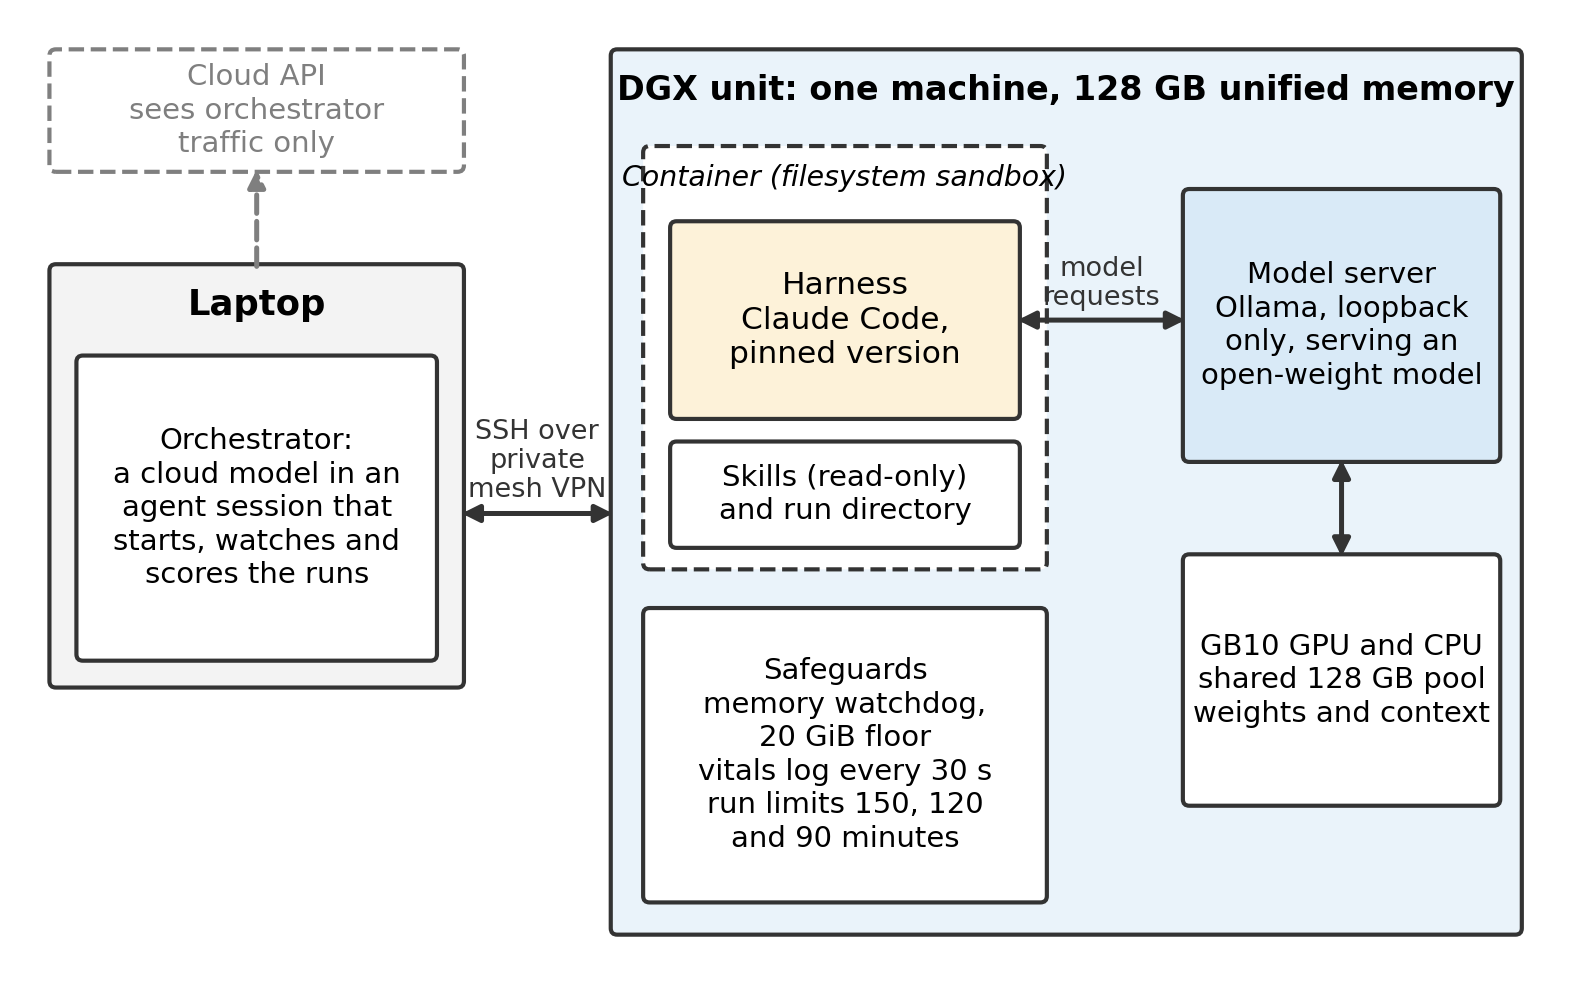
\includegraphics[width=0.85\textwidth]{figures/fig-architecture.png}
\caption{Evaluation architecture. Generation traffic (prompts and tokens) stays on the DGX; the orchestrator's supervision traffic does not. The container is a filesystem sandbox, not a network sandbox, because it shares the host network to reach the model server. No address, host name, or login appears in this paper.}
\label{fig:architecture}
\end{figure}

\subsection{Hardware and Software}

The machines are two identical NVIDIA DGX Spark-class units administered by a third party, reached from the laptop over a private mesh VPN built on WireGuard \cite{donenfeld2017wireguard, pennarun2020tailscale}. All results reported here came from one unit. Table~\ref{tab:hardware} lists the configuration.

\begin{table}[htbp]
\centering
\small
\begin{tabular}{@{}lp{12cm}@{}}
\toprule
\textbf{Component} & \textbf{Value} \\
\midrule
CPU & 20 Arm cores (10 Cortex-X925, 10 Cortex-A725) \\
GPU & NVIDIA GB10 Blackwell, 6,144 CUDA cores \\
Memory & 128~GB LPDDR5x unified, shared by CPU and GPU; 273~GB/s as published by the vendor \cite{nvidia2025dgxspark} \\
Storage & 1~TB NVMe \\
Model server & Ollama, one pinned release, installed in user space, loopback only \\
Harness & Claude Code, one pinned version, in a non-root container \\
Quantization & each publisher's default 4-bit file \\
\bottomrule
\end{tabular}
\caption{Configuration of the unit that produced every result. The GPU has no memory of its own: weights and conversation context compete for the same 128~GB as the operating system and every other program.}
\label{tab:hardware}
\end{table}

\subsection{Candidate Models}

Ten open-weight models were chosen for one 128~GB unit, in the order shown in Table~\ref{tab:models}, \textit{before} any results. The criteria came from the workload: tool calling, a context window of at least 64,000 tokens, a fit in memory with room for that context, and a publisher and license that could be identified. The order put models with early results first and then the models whose publishers' claims came closest to the two abilities the benchmark exercises. Publisher claims come from each model's library page as of October 2026 and were not checked.

\begin{table}[htbp]
\centering
\footnotesize
\begin{tabular}{@{}lrrrrl@{}}
\toprule
\textbf{Model} & \textbf{Params (B)} & \textbf{Active (B)} & \textbf{Disk (GB)} & \textbf{Window (K)} & \textbf{Decode (tok/s)} \\
\midrule
\Qeight & 27 & --- & 17 & 256 & 26$^\dagger$ \\
\Gthirtyone & 30.7 & dense & 20 & 256 & 28--40 \\
\Muse & 30 & --- & 18 & 128 & 13 \\
\Qsix & 35 & $\approx$3 & 22 & 256 & 83--105 \\
\Gtwentysix & 25.2 & 3.8 & 18 & 256 & 86--130 \\
\Nemo & 30 & 3 & 25 & 1,000 & 84--105 \\
\Mistral & 128 & dense & 80 & 256 & 3 \\
\Gptoss & 117 & 5.1 & 65 & 128 & 38--44 \\
\Devstral & 24 & --- & 15 & 384 & 15 \\
\Granite & $\approx$30 & dense & 17 & 128 & 12 \\
\bottomrule
\end{tabular}
\caption{The ten candidates. Parameters, active parameters per token, download size, and declared context window are as stated by each publisher. Decode speed is from the model-only tests with reasoning off, except $^\dagger$, which is the speed on the longest turn of that model's stage~1 harness run. A dash means the publisher's page does not state an active count. Licenses are Apache~2.0 for seven models (for \Qeight, as reported by secondary sources and not verified), a modified MIT license for \Mistral, and unstated on the library page for \Qsix{} and \Nemo.}
\label{tab:models}
\end{table}

\subsection{Protocol}

Each stage run starts from a fresh copy of its input, so no run can alter the input of another. The runner records a status file (exit code and wall-clock seconds), the full event stream, and a final result with turn and token counts. Stage 3 runs once per chapter, carrying the book written so far into each run, with a 90-minute limit per chapter and a cap of 150 turns. The server's context length was set for each model to the largest value that a linear estimate said would leave 45~GiB of memory free: 163,840 tokens for eight models and 131,072 for \Gptoss. Reasoning, where a model supports it, was left at the model's default in the harness. Sampling parameters were the server and model defaults. A memory watchdog (floor 20~GiB, GPU temperature ceiling) killed harness containers and unloaded the model before a unified-memory machine could freeze, and a vitals log recorded memory, temperature, power, and load every 30 seconds so that a freeze would leave evidence behind.

\subsection{Two Layers of Testing}

Models were tested alone before they were tested in the harness. The model-only test runs five short tasks through the server's API with no harness: Markdown writing under format rules, p5.js code, schema-constrained JSON, a tool call, and a 30,000-token prompt with a fact to retrieve. A model that cannot keep a blank line before a list fails in seconds and not after an hour. The second layer is a three-minute harness smoke test, in which the model runs the course-description-analyzer skill and the build is checked, followed by the three benchmark stages. The layers have different failure modes, which Section~\ref{sec:discussion} returns to: a model can pass the first and fail the second.

\subsection{Controlled and Uncontrolled Variables}

The independent variable is the model. Table~\ref{tab:controls} records what was held fixed and what was not. A controlled variable is a claim that must be defensible, so the table also records the ones that were not kept.

\begin{table}[htbp]
\centering
\small
\begin{tabularx}{\textwidth}{@{}lXl@{}}
\toprule
\textbf{Variable} & \textbf{How it was handled} & \textbf{Status} \\
\midrule
Course, prompts & One unchanged course description; one prompt file per stage & Controlled \\
Harness, server & Pinned Claude Code version; pinned Ollama release & Controlled \\
Skills & One checkout, read-only; a faulty example in one skill corrected before the comparison runs & Controlled \\
Hardware & One unit for all results & Controlled \\
Starting state & Fresh copy of the input for every run & Controlled \\
Time limits & 150, 120, and 90 minutes; two consecutive chapter timeouts end a model's stage~3 & Controlled \\
Quantization & Each publisher's default 4-bit file & Controlled, but differs by publisher \\
Context length & Largest that keeps 45~GiB free, per model & Uncontrolled \\
Reasoning mode & Model default in the harness; off in the model-only tests & Uncontrolled \\
Sampling & Server and model defaults & Uncontrolled \\
Server behavior & One server re-read the whole conversation on every turn; cause not found & Uncontrolled \\
Run-to-run variance & One run per model per stage & Not measured \\
Supervision & A cloud orchestrator read run output to monitor and score & Uncontrolled \\
\bottomrule
\end{tabularx}
\caption{Controlled and uncontrolled variables.}
\label{tab:controls}
\end{table}

One attempt did not follow the protocol. The first stage~1 attempt for \Gthirtyone{} ran on the second unit at a 256,000-token context and was lost when that machine stopped responding; the result reported here is the second attempt, on the first unit at 163,840 tokens. The second unit stopped responding twice, both times minutes into a run of the same model. The administrator found no recorded out-of-memory kill, GPU error, kernel panic, or thermal shutdown and reported intermittent loss of power to that unit. The cause is not established, and no result from that unit is used.
